\documentclass[pdftex, twocolumn]{article}
\usepackage{graphicx}
\usepackage{amsmath}
\usepackage{algpseudocode}
\usepackage{url}
\usepackage{amssymb}
\usepackage{bbm}
\renewcommand{\algorithmicforall}{\textbf{for each}}
\usepackage{tikz}
\usepackage{dsfont}
\providecommand{\abs}[1]{\lvert#1\rvert}
\providecommand{\Abs}[1]{\bigg\lvert#1\bigg\rvert}
\providecommand{\norm}[1]{\lVert#1\rVert}
\providecommand{\ceil}[1]{\lceil#1\rceil}
\usetikzlibrary{arrows}
\usepackage[margin=0.7in]{geometry}

\begin{document}

\author{
  Brandon Ewonus\\
  Stanford University\\
  \texttt{bewonus@stanford.edu}
  \and
  Bryan McCann\\
  Stanford University\\
  \texttt{bmccann@stanford.edu}
  \and
  Nat Roth\\
  Stanford University\\
  \texttt{nroth@stanford.edu}
}
\title{CS 229 Final Project - Party Predictor: Predicting Political Affiliation}
\date{}

\maketitle

\section*{Abstract}

\emph{In this report we analyze the political speeches made by members of the Democratic and Republican parties in the United States.  Specifically, we attempt to learn which features best differentiate speeches made by the two parties, and develop a model to classify speeches as either Democrat or Republican.}

\section{Introduction}

Division among the political parties in the United States has become an increasingly large problem. The American populace continues to recover from  the most threatening economic recession in decades. Environmental crises have plagued the nation regularly. The government shutdown, and the Treasury nearly defaulted on its debt. When members of one party bridge the divide to provide support in times of trouble, they are met with ostracization from their own party, and unfortunately polls and polarization research show that partisan divisions drive the debate amongst those who are responsible for solutions $[6]$.  What's more, the American populace does not appear to be any less divided $[7]$. 

This paper outlines a variety of supervised and unsupervised techniques employed in an effort to flesh out these divisions under the assumption that the content and rhetoric of political speeches can provide insight into the sharp divides we see in American politics today. 

\section{Data Collection and Handling}

Our dataset consists of 344 speeches (171 Republican / 173 Democrat) by American politicians delivered during or after the presidency of Franklin Roosevelt. Political lines prior to the presidency of FDR become increasingly difficult to relate in a one-to-one fashion to the political parties today; thus, we steered away from adding speeches before that time period. All of the data was collected by scraping online sources for text. The data is heavily biased towards presidents, however we have also included speeches by Congressional politicians, governors, and other major political figures to help generalize our model for the future.

Preprocessing was handled by Scikit's CountVectorizer. English stop words were removed, and CountVectorizer's defaults were used for the rest of the preprocessing, which yields word count features only.

\section{Methods / Analysis}

\subsection{Naive Bayes}

We implemented a Naive Baye�s model with Laplacian smoothing as a first step in analyzing our data. We had a nearly balanced set of 344 speeches to train on, 171 speeches coming from Republicans and 173 coming from Democrats. On this dataset, Naive Baye�s performed reasonably well, yielding a leave one out cross validation error rate of roughly 22.7\%. In addition, after training a model on the whole dataset, we examined the learned parameters to determine which words had the greatest difference in conditional probabilities. We looked at the 20 words for which we observed the maximum values of $\log(P(\text{word } i | \text{republican}) / P(\text{word } i | \text{democrat}))$, as well as the 20 words which yielded the maximum values of $\log(P(\text{word } i | \text{democrat})/P(\text{word } i |\text{republican}))$. The former gave us a list of the 20 words which were most indicative of Republican speeches, while the latter gave us the 20 words most indicative of Democratic speeches. They were as follows: 
\begin{verbatim}
Democrat: internet, algeria, bosnia, gay, assad, 
tunisia, negro, online, algerian, lgbt, barack, 
conversation, newtown, womens, ghana, secondly, 
cyber, digital, kosovo', rwanda	
\end{verbatim}

\begin{verbatim}
Republican:  russias, iraqi, conservatives, 
narcotics, abortion, iraqis, sdi, tea, heroin, 
unborn, whittier, liberals, rehabilitation, 
palin, 1974, 1982, duke, eisler, gorbachev, 
inflationary
\end{verbatim}
Some of these words, like `Barack' and `SDI' (Strategic Defense Initiative) are not as generalizable as others in terms of their predictive power; for example, the word 'Barack' is much more likely to appear in a speech by a Democrat, not necessarily because it is in inherently a more Democrat-like word, but because it is only mentioned in Obama speeches (and Obama is a Democrat). Still, many other words, like `internet' or `conservatives', match quite well with our intuition on what words Democrats and Republicans use.

\subsection{SVM}

Support Vector Machines are among the best `off-the-shelf' supervised learning algorithms available for binary classification, particularly for their efficacy when dealing with high-dimensional data such as ours where the number of feature variables (distinct words) exceeds the number of samples (documents).  In addition, SVMs offer plenty of opportunities for regularization: we can specify any valid Kernel function and soft margin penalty term.  We used the scikit-learn implementation of SVMs, as well as a built-in grid search method, to search through our set of specified regularization parameters and classify our speech documents.  We specified 4 different Kernel functions:
\begin{itemize}
\item Linear: $K(x, z) = \langle x, z \rangle$
\item Polynomial: $(\gamma \langle x, z \rangle + r)^d$
\item Radial Basis Function: $e^{-\gamma \abs{x - z}^2}$
\item Sigmoid: $\tanh(\gamma \langle x, z \rangle + r)$
\end{itemize}
Our method performed 5-fold cross-validation on our data, using each of the above Kernel functions $\big($with $d = 3$, $r = 0$, and $\gamma = \frac{1}{\text{\# features}} = \frac{1}{22135}$$\big)$ and using penalty terms $C \in \{ 1, 2, ..., 10 \}$.  The optimal kernel returned from this search was the linear function $K(x, z) = \langle x, z \rangle$, with an optimal penalty term of $C = 1$.  The training error for these specific parameters was 0\% with a cross-validation error of 24.7\%.

\subsection{Logistic Regression}

We fit a regularized logistic regression model as well. We tried both L1 and L2 regularization, with varying degrees of strength. We observed the best performance  at 24.13\% LOOCV,  using L1 regularization and with regularization at the inverse of .5.  When we decreased the penalty, performance decreased. This was expected, since our dataset consists of only 344 data points, but has around 22135 unique words of features. So without strong regularization, we overfit on our train set and thus see a worse test error. When we rank speeches by leaving one out, the most democratic speeches were given by the Clinton's and President Obama. The most republican speeches were more spread across the Republican party and included Nixon, Ford, and Reagan.

\subsection{LDA}

In each of the machine learning algorithms above, we used the entire word count matrix to classify documents, using optimized regularization to reduce the number of feature variables.  We decided to use Linear Discriminant Analysis to find the linear combination of features which best explains the variance between the two parties.  With only one component, we obtain a LOOCV error of 22.5\%, which is nearly identical to our performance using the methods above.  Our training error was 11.4\%.  A plot of the speeches is shown in Figure 1.  Since only one component was used to separate the data (x-axis), we added uniform noise to the data (y-axis) for easier visualization.

\begin{figure}[h!]
\centering
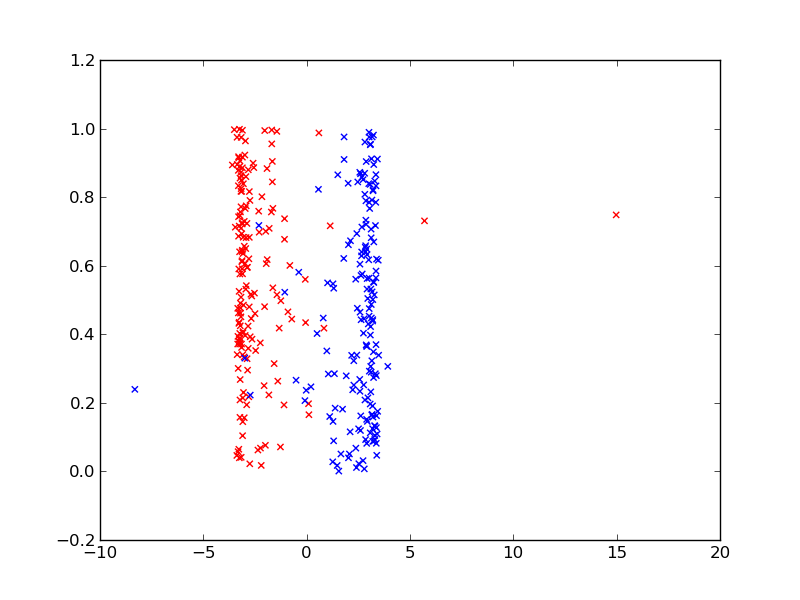
\includegraphics[scale=0.4,width=0.5\textwidth]{VFLDA.png}
\caption{LDA plot of Republicans (red) and Democrats (blue).  The data are jittered in the vertical direction with uniform noise for ease of visualization.}
\centering
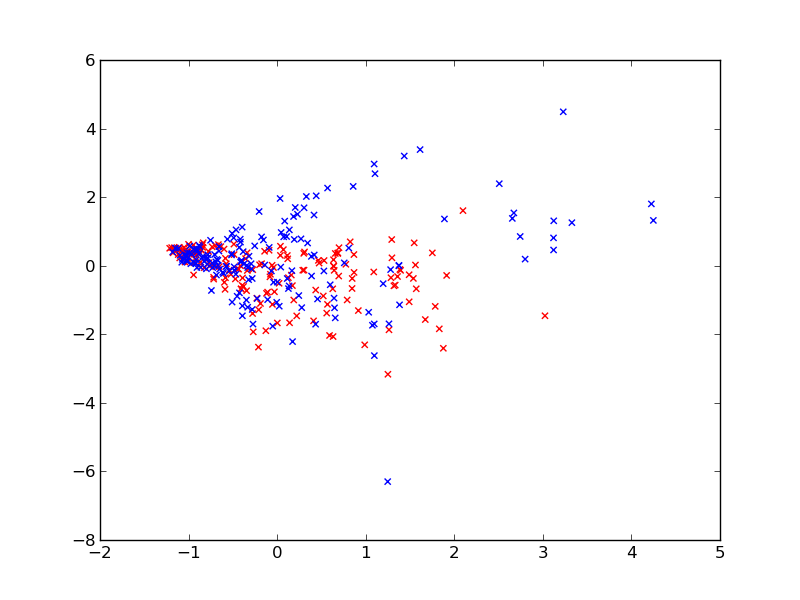
\includegraphics[scale=0.4,width=0.5\textwidth]{VFPCA.png}
\caption{PCA plot of Republicans (red) and Democrats (blue) onto the first two principal components.}
\end{figure}

\subsection{PCA}

To gain further insight into the data, we used principal component analysis to reduce the dimensionality of our data, which works by finding the set of $k$ mutually orthogonal features which best explain the variation in the overall data (not taking party labels into account).  We made a PCA plot of the data, with the x and y axes representing the first and second components respectively, and colored points based on political party.  We noticed that some speeches, namely 

Specifically, we computed $k$ principal components for each $k \in \{ 1, ..., 50 \}$, and then ran logistic regression using the $k$ features from PCA (using L1 regularization with a very minimal penalty).  The leave one out cross validation error was recorded for each $k$.  Remarkably, with $k$ as small as 8 we achieved a LOOCV error of $21\%$, and with $k = 23$ we achieved nearly the same LOOCV error as with the methods above ($16\%$).  One drawback of using PCA is that the interpretation of what the $k$ components represent may be somewhat challenging, however the fact that we can achieve similar performance and accuracy as may other supervised learning methods with far fewer features is exciting.  In the future, we plan to plot the documents along the first two principal components in order to see what underlying structure is present, and which documents help define these 2 axes.  We will also consider utilizing LDA or QDA as additional dimensionality reduction algorithms, which may be better suited for binary classification than PCA (since they search for the linear combinations of features which best explain the variance \emph{between} classes).

\begin{figure}[h!]
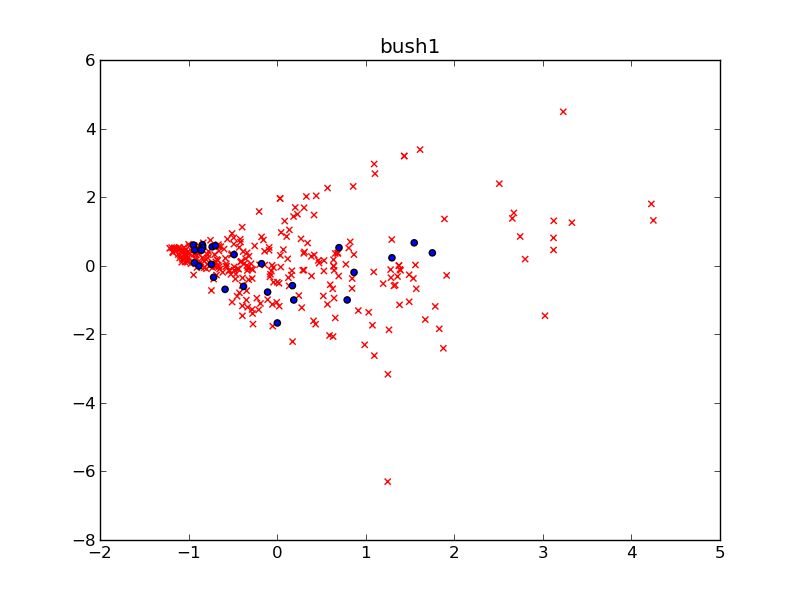
\includegraphics[scale=0.2]{bush1_pca.png}
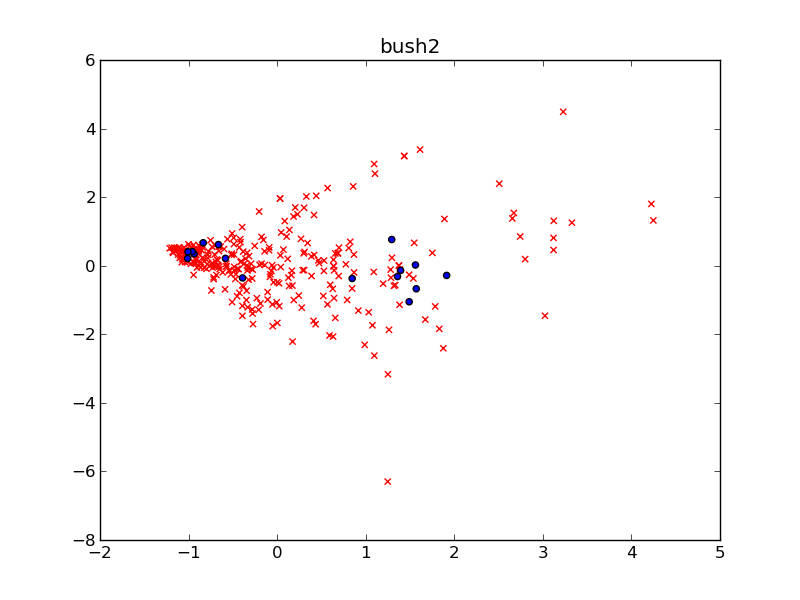
\includegraphics[scale=0.2]{bush2_pca.png}
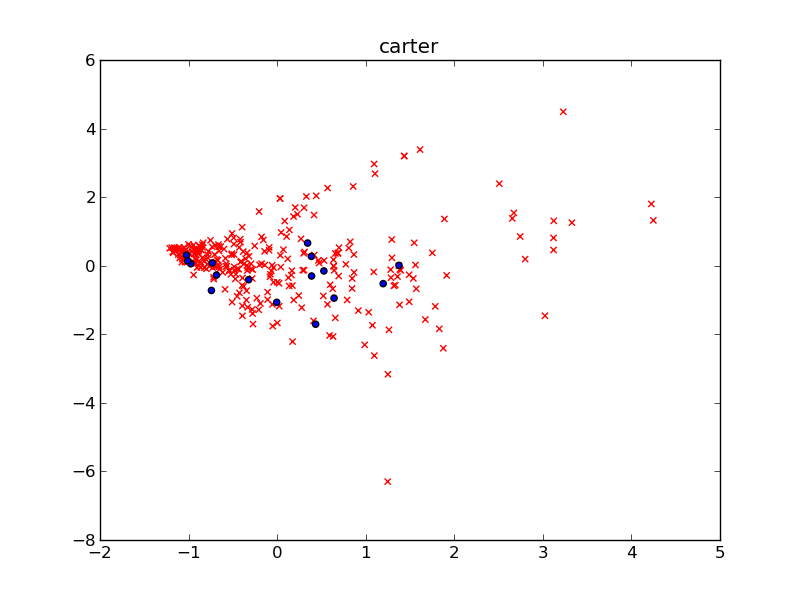
\includegraphics[scale=0.2]{carter_pca.png}
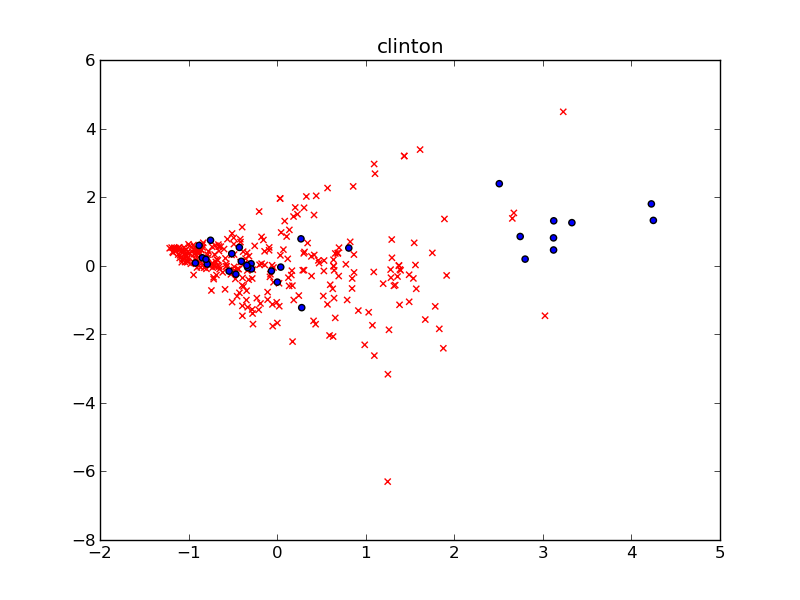
\includegraphics[scale=0.2]{clinton_pca.png}
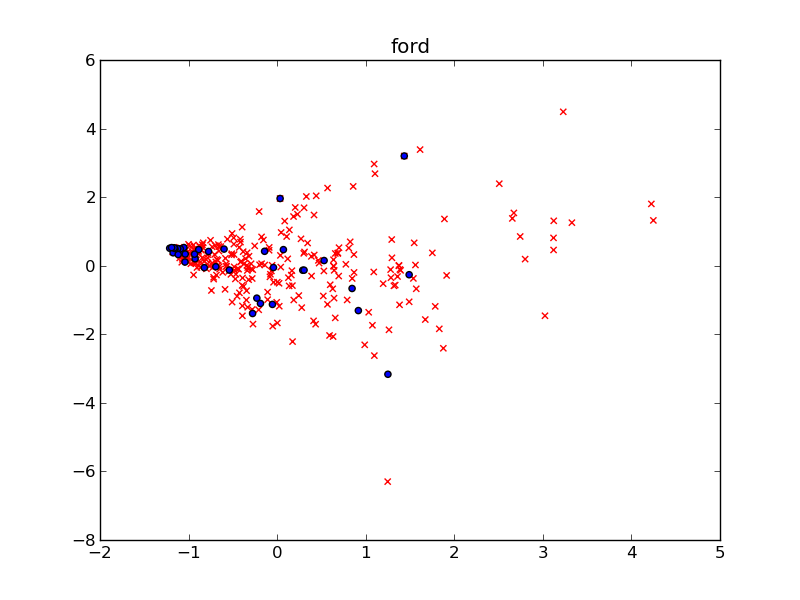
\includegraphics[scale=0.2]{ford_pca.png}
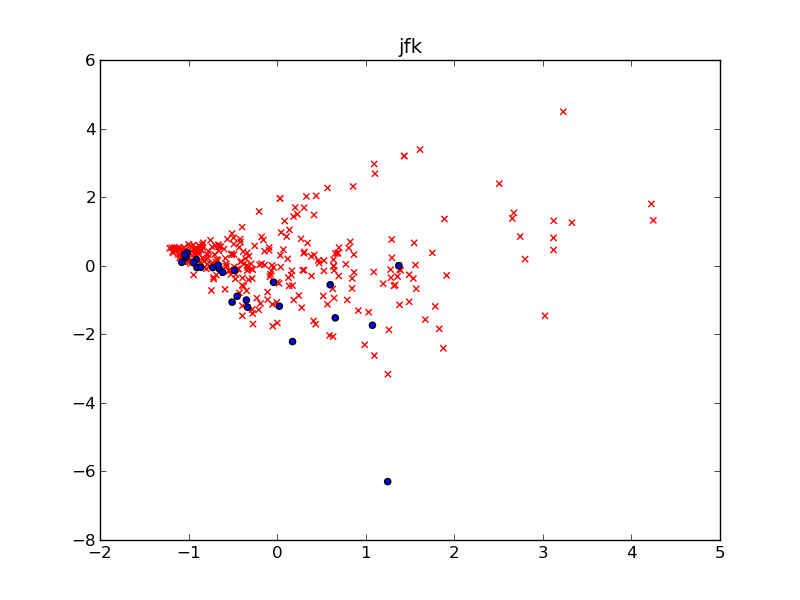
\includegraphics[scale=0.2]{jfk_pca.png}
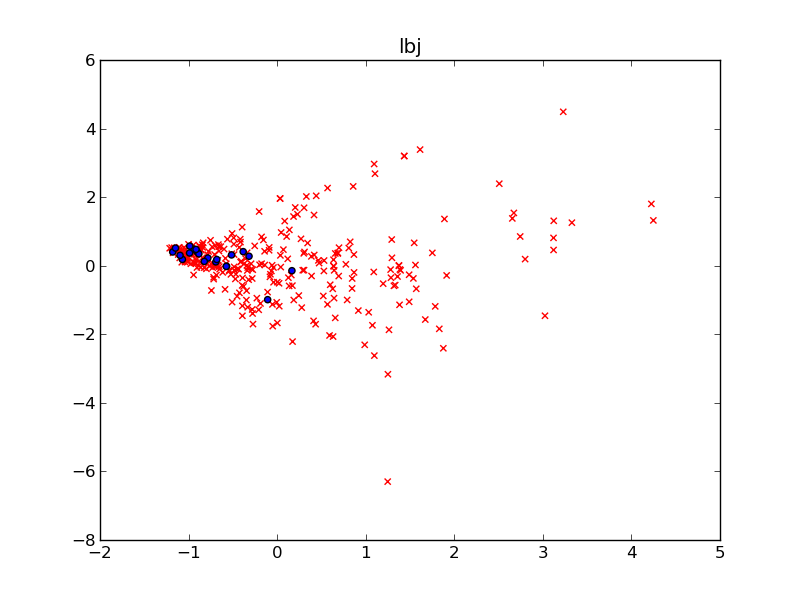
\includegraphics[scale=0.2]{lbj_pca.png}
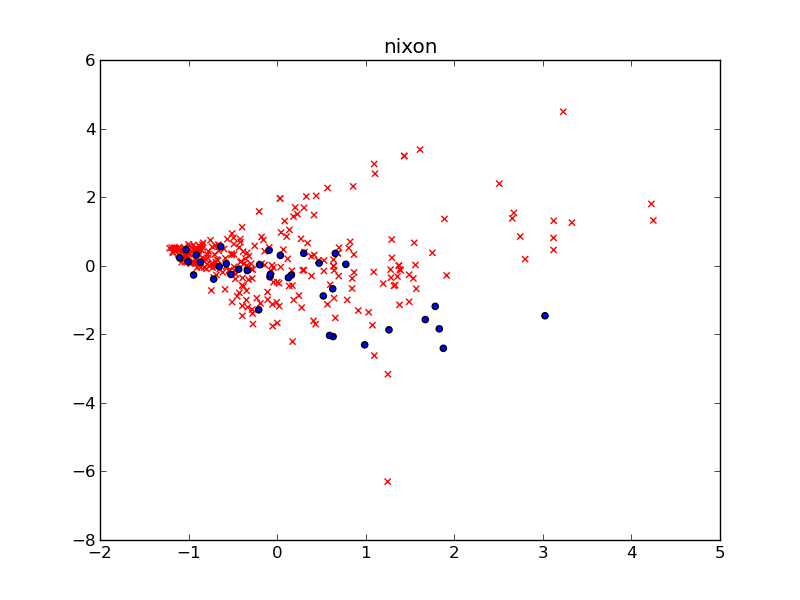
\includegraphics[scale=0.2]{nixon_pca.png}
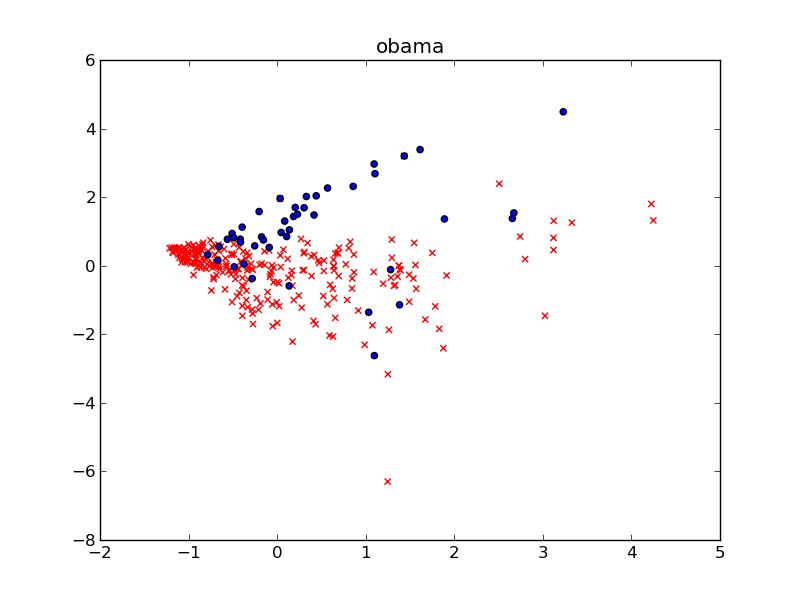
\includegraphics[scale=0.2]{obama_pca.png}
\hspace{1.1pc}
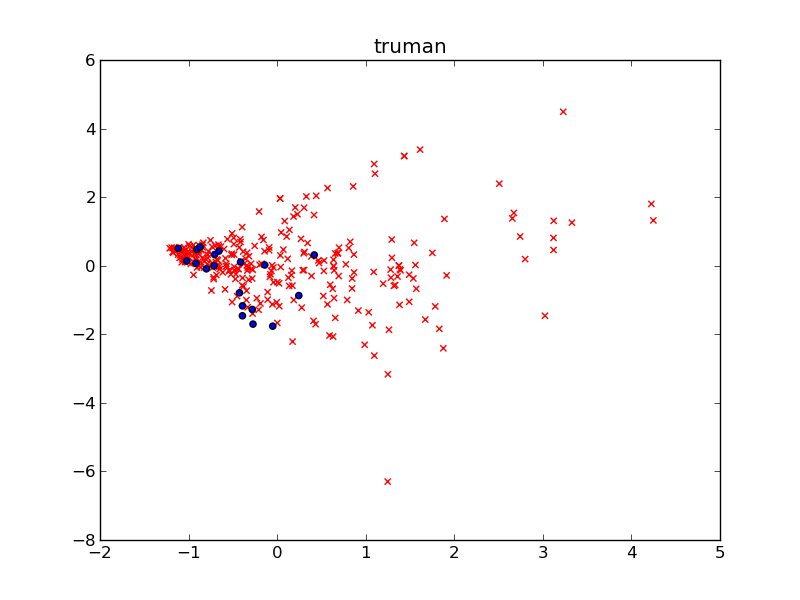
\includegraphics[scale=0.2]{truman_pca.png}
\caption{PCA plots with specific presidents highlighted.  Notice in particular the plots associated with Clinton, Nixon, and Obama, which together seem to contain most of the outliers from the overall plot.}
\end{figure}

\subsection{K-means}

In addition to using supervised learning algorithms for classification, we also ran K-means on our data in order to determine whether there were any inherent clustering patterns among the speeches we analyzed.  We expected to see divides based on political party, however we were also interested to see which other trends might be present in the data.  With 8 clusters, the documents separated as follows:

\vspace{1pc}
\noindent
Cluster 1: 12 Obama, 1 Palin

\vspace{1pc}
\noindent
Cluster 2: 8 Clinton, 1 Obama

\vspace{1pc}
\noindent
Cluster 3: 6 Nixon

\vspace{1pc}
\noindent
Cluster 4: 1 Clinton

\vspace{1pc}
\noindent
Cluster 5: 1 JFK

\vspace{1pc}
\noindent
Cluster 6: 1 JFK

\vspace{1pc}
\noindent
Cluster 7: 80 speeches; 55 Republican, 25 Democrat

\vspace{1pc}
\noindent
Cluster 8: 233 speeches; 109 Republican, 124 Democrat

\vspace{1pc}
\noindent
Interestingly, the first three clusters listed above consist almost entirely of one president each, either Obama, Clinton, or Nixon (compare this with the PCA plots in Figure 3).  The next three clusters contain a single speech each, and the last two contain all of the remaining speeches.  The clusters also seemed to be somewhat topically organized.  The Obama speeches in Cluster 1 pertain mostly to the economy, affordability, and employment.  All of Clinton's speeches (and Obama's as well) in Cluster 2 are state of the union addresses.  Nixon's speeches in Cluster 3 are mostly press conference or convention talks, and concern leadership.  Cluster 4 regards health care reform, Cluster 5 is about imperialism, and Cluster 6 is about taxation.  Clusters 7 and 8 contained no obvious patterns, other than that a reasonable majority of the speeches in cluster 7 are Republican speeches, many of which are state of the union addresses.  Running K-means with fewer than 8 clusters didn't divide the data significantly, and running K-means with more than 8 clusters didn't seem to add any more insights (other than stripping away individual speeches from one of the larger two clusters).

\subsection{K-Nearest Neighbors}

FILL THIS IN.

\section{Results}

\subsection{Unsupervised Insights}

 Most of the speeches we analyzed are similar to each other. Many speeches by Obama and Clinton (and Nixon to some extent) stand out from the rest, and from each other. There tends to be greater variability among Democrat speeches than there is among Republican speeches

\subsection{Presidential Rankings}

In order to rank our presidents by political affiliation, we, for each pair of (Democrat, Republican) presidents, held out the training examples for those presidents, and then obtained the probability of each president being Democrat. We used a president�s average probability of being Democrat to sort our rankings.  We also calculated the proportion of times that we correctly identified the Democrat as more of a Democrat than the Republican. We called this the H2H (Head-to-Head) score. 

In order of most to least Democrat: 1. Nixon 2. Bush Sr. 3. Truman 4. Ford 5. Carter 6. Clinton 7. JFK 8. LBJ 9. Reagan 10. Obama 11. Bush

Looking at these rankings, one can clearly see that this ordering is simply not accurate. Our final H2H score was  53.3\%, indicating that we did little better than chance. Combining this with the PCA plots, we suspected that our high accuracies in supervised learning were not a result of  political affiliation. Rather, it resulted from learning enough about an individual�s speech style to associate that back to political party. 

\section{Conclusion}

FILL THIS IN.

\begin{thebibliography}{9}

\bibitem{lamport94}
  ``scikit-learn: Machine Learning in Python''.
  
  $<$\url{http://scikit-learn.org/stable/index.html}$>$

\bibitem{lamport94}
  ``History \& Politics Out Loud: Famous Speeches''.
  
  $<$\url{http://www.wyzant.com/resources/lessons/history/hpol/}$>$
  
\bibitem{lamport94}
  ``American Rhetoric Speech Bank''.
  
  $<$\url{http://www.americanrhetoric.com/}$>$

\bibitem{lamport94}
  ``Presidential Rhetoric''.
  
  $<$\url{http://www.presidentialrhetoric.com}$>$

\bibitem{lamport94}
  ``The American Presidency Project''.
  
  $<$\url{http://www.presidency.ucsb.edu/index.php#axzz2i2nXPc43}$>$

\bibitem{lamport94}
  ``Partisan Polarization Surges in Bush, Obama Years''.
  
  $<$\url{http://www.people-press.org/2012/06/04/partisan-polarization-surges-in-bush-obama-years/}$>$

\bibitem{lamport94}
  ``Political partisanship mirrors public''.
  
  $<$\url{http://www.usatoday.com/story/news/politics/2013/03/06/partisan-politics-poll-democrats-republicans/1965431/}$>$

\end{thebibliography}

\end{document}